\documentclass{report}
\usepackage[utf8]{inputenc}

\title{Bases formelles du TAL \\ corrections d'exercices}
\author{Pierre-Léo Bégay}
%\date{October 2019}

\usepackage{natbib}
\usepackage{graphicx}
\usepackage{hyperref}
\usepackage{soul}
\usepackage{amssymb}
\usepackage{amsmath}
\usepackage{tikz}
\usepackage{subcaption}
\usepackage{tikz-qtree}
\usepackage{tikz-qtree-compat}
\usepackage{graphbox}
\usepackage{tabularx}
\usepackage{stmaryrd}
\usepackage{float}


\usetikzlibrary{arrows,automata}
\tikzset{initial text={}}
\usetikzlibrary{calc,shapes.multipart,chains,arrows}

 

\newcommand{\mt}[1]{\left\llbracket \vcenter{
     \hbox{\bfseries#1}} \right\rrbracket}

\usepackage[a4paper]{geometry}


\hypersetup{
    colorlinks=true,       % false: boxed links; true: colored links
    linkcolor=blue,          % color of internal links (change box color with linkbordercolor)
    citecolor=blue,        % color of links to bibliography
    filecolor=magenta,      % color of file links
    urlcolor=cyan           % color of external links
}
\usepackage{pythonhighlight}
\usepackage{parskip}
\setlength{\parskip}{0.5em}
\setlength{\parindent}{0pt}%
\usepackage{amsthm}
\usepackage{epigraph}
\setlength{\epigraphwidth}{0.6\textwidth}
%\theoremstyle{definition}
%\newtheorem{definition}{Définition}[section]

\newtheoremstyle{slanted}
  {1em plus .2em minus .1em}%   Space above
  {1em plus .2em minus .1em}%   Space below
  {\slshape}%  Body font
  {}%          Indent amount (empty = no indent, \parindent = para indent)
  {\bfseries}% Thm head font
  {.}%         Punctuation after thm head
  {0.5em}%     Space after thm head: " " = normal interword space;
     %         \newline = linebreak
  {}%          Thm head spec (can be left empty, meaning `normal')

\theoremstyle{slanted}

\newtheorem{example}{Exemple}[section]
\newtheorem{exercice}{Exercice}[section]
\newtheorem*{correction*}{Correction}

\usepackage{tcolorbox}
\tcbuselibrary{theorems}


\newtcbtheorem[number within=section]{definition}{Définition}%
{colback=blue!10,colframe=blue!30!black,fonttitle=\bfseries}{th}

%\newtcbtheorem[number within=section]{lemma}{Lemme}%
%{colback=green!10,colframe=blue!30!black,fonttitle=\bfseries}{th}

\begin{document}

\maketitle


\tableofcontents


\chapter{Langages}
\label{langages}

On définit d'abord la notion de mot, nécessaire à celle de langage. On verra ensuite comment décrire des langages à l'aide de notations ensemblistes, révisant ces dernières par la même occasion.

\section{Mots}

\begin{definition}{Mot}{}Un \textbf{mot} est une suite de lettres tirées d'un alphabet donné. L'ensemble des mots sur un alphabet $\Sigma$ est noté $\Sigma^*$.
\end{definition}

\begin{example}
Etant donné l'alphabet $\Sigma = \{a,b,c\}$, on peut construire une infinité de mots parmi lesquels 

\begin{itemize}
    \item $abc$
    \item $aab$
    \item $cc$
    \item $abcabcacbacbacbacbabcabcabcabcabcabcabc$
    \item $a$
\end{itemize}

\end{example}


\paragraph{Remarque} On va s'intéresser ici à des langages et mots complètement abstraits, en général composés uniquement de $a$, $b$ et $c$.

\begin{definition}{Mot vide}{}
Une suite de lettres peut être de longueur zéro, formant alors \textbf{le mot vide}. Quel que soit l'alphabet, ce dernier sera noté $\epsilon$.
\end{definition}

\begin{definition}{Concaténation}{}
\label{concat}
L'opération de \textbf{concaténation}, notée $.$, consiste tout simplement à "coller" deux mots.
\end{definition}

\begin{example}{Quelques concaténations :}

\begin{itemize}
    \item $ab.c = abc$
    \item $ab.ba = abba$
\end{itemize}
\end{example}

 De plus, pour tout mot $w$, 

\[
    w.\epsilon = \epsilon.w = w
\]

\paragraph{Remarque} Les algébristes enthousiastes remarqueront que $(\Sigma^*,.,\epsilon)$ forme un monoïde libre de base $\Sigma$


\begin{definition}{Longueur d'un mot}{}
Etant donné un mot $w$, on note sa \textbf{longueur} $|w|$.
\end{definition}

\begin{example}
Tout naturellement,
\begin{itemize}
    \item $|abc| = 3$
    \item $|abba| = 4$
    \item $|c| = 1$
    \item $|\epsilon| = 0$
\end{itemize}
\end{example}

\begin{definition}{Principe d'induction sur un mot}{}
Etant donnée une propriété $P$ sur les mots. Si on a\\

\begin{enumerate}
\item $P(\epsilon)$ (cad. que $P$ est vraie pour le mot vide)
\item $\forall w, \forall c \in \Sigma, (P(w) \rightarrow P(c.w))$ (cad. que si $P$ est vraie pour un mot, alors elle reste vraie si on rajoute n'importe quelle lettre à gauche du mot)\\
\end{enumerate}

Alors la propriété $P$ est vraie pour tout mot $w$.
\end{definition}

\paragraph*{Remarque} Est également valide le principe d'induction où, dans le cas récursif, la lettre est rajoutée à droite du mot plutôt qu'à sa gauche.


\begin{definition}{Nombre d'occurrences d'une lettre}{}
Etant donné un mot $w$ et une lettre $a$, on note $\mathbf{|w|_a}$ le nombre de $a$ dans $w$.
\end{definition}

\begin{example}
On a 
\begin{itemize}
    \item $|abc|_a = 1$
    \item $|abba|_b = 2$
    \item $|c|_a = 0$
    \item $|\epsilon|_a = 0$
\end{itemize}
\end{example}

\begin{definition}{Préfixe}{}
Un mot $p$ est un \textbf{préfixe} du mot $w$ ssi $\exists v, w = p.v$, cad. ssi $w$ \textit{commence} par $p$.
\end{definition}

\begin{definition}{Suffixe}{}
Un mot $s$ est un \textbf{suffixe} du mot $w$ ssi $\exists v, w = v.s$, cad. ssi $w$ \textit{finit} par $p$.
\end{definition}

\begin{example}
Le mot $abba$ admet comme préfixes $\epsilon$, $a$, $ab$, $abb$ et $abba$. Ses suffixes sont, quant à eux, $\epsilon$, $a$, $ba$, $bba$ et $abba$.
\end{example}

\begin{lemma}
$\forall w \in \Sigma^*, \epsilon$ et $w$ sont des préfixes de $w$
\end{lemma}
 
\begin{proof}
Pour $\epsilon$, il suffit de prendre $v = w$. A l'inverse, en prenant $v = \epsilon$, on voit que $w$ est son propre préfixe.
\end{proof}

\begin{lemma}
$\forall w \in \Sigma^*, \epsilon$ et $w$ sont des suffixes de $w$
\end{lemma}

\begin{proof}
Analogue au lemme précédent.
\end{proof}


\begin{exercice}\label{expref}
Combien de préfixes et suffixes admet un mot $w$ quelconque ?
\end{exercice}

\begin{definition}{Facteur}{}
Un mot $f$ est un \textbf{facteur} du mot $w$ ssi $\exists v_1 v_2, w = v_1.f.v_2$, cad. ssi $f$ apparaît dans $w$.
\end{definition}

\begin{example}
Les facteurs du mot $abba$ sont $\epsilon$, $a$, $b$, $ab$, $ba$, $abb$, $bba$ et $abba$. 
\end{example}

\begin{lemma}
$\forall w \in \Sigma^*$, $\epsilon$ et $w$ sont des facteurs de $w$.
\end{lemma}

\begin{proof}
Pour $\epsilon$, il suffit de prendre $v_1 = w$ et $v_2 = \epsilon$ (ou l'inverse) et la condition est trivialement vérifiée. Pour $w$, on prend $v_1 = v_2 = \epsilon$.
\end{proof}

\begin{exercice}
Donner l'ensemble des facteurs du mot $abbba$.
\end{exercice}

\begin{exercice} \label{exfact}(*)
Donner la borne la plus basse possible du nombre de facteurs d'un mot $w$. Donner un mot d'au moins 3 lettres dont le nombre de facteurs est exactement la borne donnée.
\end{exercice}

\begin{definition}{Sous-mot}{}
Un mot $s$ est un \textbf{sous-mot} du mot $w$ ssi $w = v_0s_0v_1s_1v_2...s_nv_n$ et $s = s_0s_1...s_n$, cad. ssi $w$ est "$s$ avec (potentiellement) des lettres en plus".
\end{definition}

\begin{example}\label{ex5} On \underline{souligne} les lettres originellement présentes dans le sous-mot :
\begin{itemize}
   \item $ab$ est un sous-mot de $b\underline{a}a\underline{b}$, qu'on pourrait aussi voir comme $ba\underline{ab}$
   \item $abba$ est un sous-mot de $ba\underline{a}abaa\underline{bb}a\underline{a}$.
   \item $ba$ \underline{n}'est \underline{pas} un sous-mot de $aaabbb$ (l'ordre du sous-mot doit être préservé dans le mot) 
\end{itemize}
\end{example}


\begin{lemma}
$\forall w \in \Sigma^*$, $\epsilon$ et $w$ sont des sous-mots de $w$.
\end{lemma}

\begin{proof}
Pour $\epsilon$, il suffit de prendre $n = 0$, $s_0 = \epsilon$, $v_0 = w$ et $v_1 = \epsilon$ (ou l'inverse) et la condition est trivialement vérifiée. Pour $w$, on prend $n = 0$, $s_0 = w$ et $v_0 = v_1 = \epsilon$.
\end{proof}

\begin{exercice}
Montrer que tout facteur d'un mot en est également un sous-mot. A l'inverse, montrer qu'un sous-mot n'est pas forcément un facteur. 
\end{exercice}

\begin{exercice}
Donner toutes les façons de voir $abba$ comme sous-mot de $baaabaabbaa$ (cf. exemple \ref{ex5}).
\end{exercice}

\begin{exercice}
Donner l'ensemble des sous-mots de $abba$
\end{exercice}

\begin{exercice}\label{exssmot} (*)
Donner la borne la plus basse possible du nombre de sous-mots d'un mot $w$. Donner un mot dont le nombre de sous-mots est exactement la borne donnée.
\end{exercice}

\begin{exercice} (*) Dans l'exercice \ref{expref}, on demande le nombre exact de préfixes et suffixes d'un mot, alors que dans les exercices \ref{exfact} et \ref{exssmot}, on demande une borne, pourquoi ?
\end{exercice}

\section{Langage}

\begin{definition}{Langage}{}
Un langage, c'est un ensemble de mots. 
\end{definition}

On distingue donc d'entrée les deux langages extrêmes : $\mathbf{\Sigma^*}$, l'ensemble (infini) de tous les mots formés à partir de $\Sigma$, et $\mathbf{\emptyset}$, le langage / ensemble vide, qui se caractèrise comme ne contenant aucun élément.

\paragraph{Remarque} Ne surtout pas confondre $\emptyset$ et $\{\epsilon\}$. Le premier est un ensemble vide, contenant donc \textbf{0} élément, trandis que le second contient \textbf{1} élément, le mot ide. 

La question maintenant est maintenant de savoir comment on définit et parle de langages précis et plus "intermédiaires" que les deux précédents. En tout généralité, les ensembles peuvent être définis de façon \textbf{extensionnelle} ou \textbf{intentionnelle}. 

\begin{definition}{Définition extensionnelle d'un ensemble}{}
On \textbf{définit extensionnellement un ensemble} en en donnant la liste des éléments. L'ensemble vide se note quant à lui $\emptyset$.
\end{definition}

\begin{example} On définit par exemple l'ensemble (sans intérêt) suivant :
\[
    A = \{b, aca, abba\}
\]
\end{example}

Les définitions extensionnelles ont le mérite d'être pour le moins simples, mais pas super pratiques quand il s'agit de définir des ensembles avec un nombre infini d'éléments, comme l'ensemble des mots de longueur pair. 

\begin{definition}{Définition intensionnelle d'un ensemble}{}
On \textbf{définit intensionnellement un ensemble} à l'aide d'une propriété que tous ses éléments satisfont. Étant donnés une propriété $Q(x)$ (typiquement représentée sous la forme d'une formule logique) et un ensemble $A$, on note $\{x \in A~|~Q(x)\}$ l'ensemble des éléments de $A$ qui satisfont $P$. Si l'ensemble $A$ est évident dans le contexte, on s'abstiendera de le préciser.
\end{definition}

\begin{example}
On peut définir l'ensemble des mots de longueur paire $\{w \in \Sigma^*~|~|w|~pair\}$.
\end{example}

Si les définitions intentionnelles permettent, contrairement aux extensionnelles, de dénoter des ensembles contenant une infinité de mots, elles sont avant tout un outil théorique. En effet, une propriété comme "$|w|$ paire" ne dit rien à un ordinateur en soi, et doit donc être définie formellement. Se pose alors la question d'un langage pour les propriétés.

Plusieurs logiques équipées des bonnes primitives peuvent être utilisées, mais les traductions sont rarement très agréables. Certaines propriétés nécessitent en effet de ruser contre le langage, voire sont impossibles à formaliser dans certaines logiques. Il existe heureusement un outil qui va nous aider, avec le premier problème du moins.

\chapter{Expressions régulières}
\label{regex}
Les expressions régulières permettent définir de façon finie - et relativement intuitive - "la forme" des mots d'un langage, potentiellement infini. On en présentera d'abord le lexique et l'idée générale à l'aide d'exemples, puis on en définira formellement la syntaxe et la sémantique.


\chapter{Expressions régulières}
\label{regex}

\section{Lexique et idée générale}

\subsection{Les lettres et $\epsilon$, la base}

\subsection{$.$, la concaténation}

\subsection{*, l'itération}

\begin{exercice}
Donner 5 autres mots appartenant au langage dénotée par l'expression de l'exemple \ref{ex1}. 
\end{exercice}

\begin{exercice}
Pourquoi le changement de formulation dans les exemples \ref{ex0} et \ref{ex1} par rapport aux exemples précédents ("c'est à dire $\{x, y, z ... \}$" qui devient "contenant notamment $x$, $y$ ou $z$") ?
\end{exercice}

\subsection{$+$, la disjonction}

\begin{exercice}
Donner un mot acceptant deux dérivations avec la regex de l'exemple \ref{ex3} (justifier en donnant les dérivations). Existe-t-il un autre mot admettant plusieurs dérivations ?
\end{exercice}

\begin{exercice}
Existe-t-il un mot acceptant plusieurs dérivations pour la regex de l'exemple \ref{ex4} ?
\end{exercice}

\begin{exercice}
Donner un mot accepté par la regex de l'exemple \ref{ex4} mais pas celle de l'exemple \ref{ex3}. Est-il possible de trouver un mot qui, à l'inverse, est accepté par la deuxième mais pas la première ?
\end{exercice}


\begin{exercice} (*)
Exprimer, en langue naturelle et de façon concise, le langage dénoté par la regex de l'exemple \ref{ex2}. Traduire ensuite ce langage en une regex non-ambiguë, c'est-à-dire où il n'y aura qu'une dérivation pour chaque mot.
\end{exercice}

\section{Syntaxe}


\section{Sémantique}
\label{resem}

\subsection{Les cas de base}

\subsection{Sémantique de la concaténation}

\subsection{Sémantique de la disjonction}

\subsection{Sémantique de l'itération}


\section{Mise en application}

\subsection{Quelques astuces}

\begin{exercice}
Donner une \textit{regex} pour les mots qui commencent par $a$.
\end{exercice}

\begin{exercice}
Donner une \textit{regex} pour les mots qui finissent par $b$.
\end{exercice}

\begin{exercice}
Donner une \textit{regex} pour les mots qui commencent par $a$ finissent par $b$.
\end{exercice}


\begin{exercice}
Donner une \textit{regex} pour les mots de longueur paire.
\end{exercice}

\begin{exercice}
Donner une \textit{regex} pour les mots de longueur impaire qui contiennent au moins 4 lettres.
\end{exercice}

\begin{exercice}
Donner une \textit{regex} pour les mots de longueur impaire, qui contiennent au moins 4 lettres, comment par $a$ et finissent par $b$.
\end{exercice}


\subsection{Syntaxe en pratique}




\chapter{Automates finis}
\label{automates}


%\epigraph{- "Qu'est-ce qu'un automate ?"\\- "Des ronds et des flèches m'sieur !"\\- "Rien à voir ! [...] Un automate, c'est un graphe orienté."}{[censuré]}

Les automates forment un langage de programmation un peu particulier, en ce qu'il est très visuel (chaque programme est un graphe annoté, ou plus prosaïquement des ronds et des flèches) et que tout programme a le même type : un mot en entrée, un booleen en sortie. Un automate définit donc un langage en donnant un moyen automatique de déterminer si n'importe quel mot donné en fait partie ou non\footnote{En ce sens, les automates sont des \href{https://fr.wikipedia.org/wiki/Fonction_caract\%C3\%A9ristique_(th\%C3\%A9orie_des_ensembles)}{fonctions caractéristiques}, qui sont aux ensembles ce que les videurs sont aux boîtes de nuit.}.

Les automates se divisent en de nombreuses sous-catégories, dont certaines ramifications seront explorées dans ce cours. On verra d'abord le fonctionnement général des automates finis déterministes (\ref{DFA}) et non-déterministes (\ref{NDFA}), en allant à chaque fois du général au technique. On verra ensuite des algorithmes pour transformer (\ref{transauto}) des automates. On étudiera enfin les combinaisons d'automates, et donc les propriétés de clôture des langages qu'ils définissent (\ref{cloture}).

\section{Automates finis déterministes}
\label{DFA}

On introduit les Automates finis déterministes, noté $AFD$ (ou $DFA$, pour \textit{deterministic finite automaton}\footnote{Notez qu'on parle d'\textit{automat\textbf{on}} au singulier et d'\textit{automat\textbf{a}} au pluriel}), avant d'en étudier la formalisation.


\subsection{Principe général}

Imaginez que vous développiez un jeu d'infiltration. Dans ce jeu, le comportement des méchants gardes ressemblerait sans doute à la figure \ref{garde}.

\begin{figure}[!h]
\centering
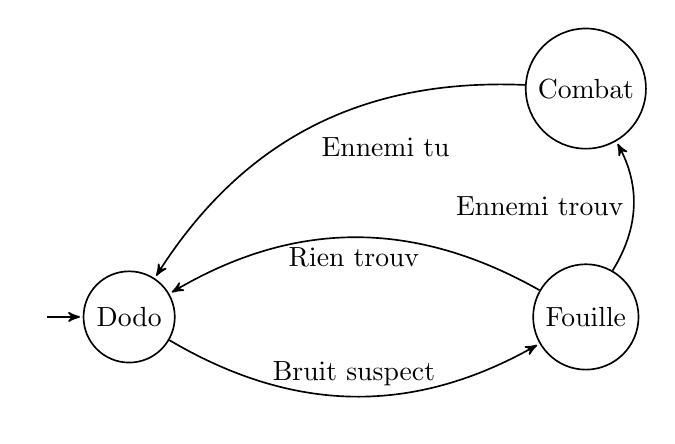
\begin{tikzpicture}[->,>=stealth',shorten >=1pt,auto,node distance=2.9cm,
                    semithick]
  \tikzstyle{every state}=[fill=white,text=black]
  \tikzstyle{place}=[rectangle,draw=black,fill=white, minimum size=7mm]


  \node[initial,state] (A)                    {Dodo};
  \node[] (D) [right of=A] {} ;
  \node[state] (B)      [right of=D]                {Fouille};
  \node[state] (C)      [above of=B]                {Combat};

  \path %(I) edge[loop above]              node {$a,b$} (I)
(A) edge      [bend right]        node {Bruit suspect} (B)
(B) edge      [bend right]        node {Rien trouvé} (A)
(B) edge      [bend right]        node {Ennemi trouvé} (C)
(C) edge      [bend right]        node {Ennemi tué} (A);
\end{tikzpicture}
\caption{Comportement des gardes d'un jeu imaginaire}
\label{garde}
\end{figure}

Ce qu'est censé traduire ce graphe, c'est qu'un garde commence (la $\rightarrow$ sur sa gauche) dans un \textbf{état} qui est le dodo, et que différents événements (un bruit, un ennemi trouvé ou non, ou encore tué) vont le faire changer d'\textbf{état}. Un AFD fonctionne sur un principe similaire\footnote{Les AFD sont en fait des cas particuliers de Machines à états finis, \href{https://www.youtube.com/watch?v=JyF0oyarz4U}{qui sont effectivement employées dans la conception de jeux vidéo}}, mais où les transitions sont déclenchées par la lecture de lettres : un $AFD$, en partant d'un état initial, lit le mot donné en argument lettre par lettre et, à chaque lecture, change d'état en fonction de la lettre. 

\begin{example}
L'automate de la figure \ref{aaauto} contient trois états, appelés $0$, $1$ et $2$. La lecture de tout mot commence en $0$, appelé \textbf{état initial}. Si on lui passe le mot $abbaaba$ en argument, la première lettre ($a$) va nous faire passer de l'état $0$ à $1$. La deuxième lettre ($b$) nous refait passer en $0$. La troisième ($b$) nous y fait rester. Les deux lettres suivantes nous font ensuite passer en $1$ puis en $2$. Les deux dernières lectures nous font rester en $2$ (la virgule est à comprendre comme une disjonction, cad. comme un "ou").
\end{example}



\begin{figure}[!h]
\centering
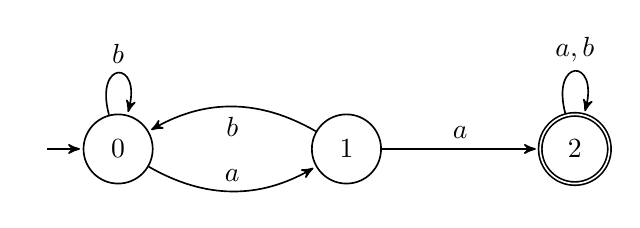
\begin{tikzpicture}[->,>=stealth',shorten >=1pt,auto,node distance=2.9cm,
                    semithick]
  \tikzstyle{every state}=[fill=white,text=black]
  \tikzstyle{place}=[rectangle,draw=black,fill=white, minimum size=7mm]


  \node[initial,state] (A)                    {$0$};
  \node[state] (B)      [right of=A]                {$1$};
  \node[accepting,state] (C)      [right of=B]                {$2$};

  \path %(I) edge[loop above]              node {$a,b$} (I)
(A) edge      [loop above]        node {$b$} (A)
(C) edge      [loop above]        node {$a,b$} (C)
(A) edge      [bend right]        node {$a$} (B)
(B) edge      [bend right]        node {$b$} (A)
(B) edge      []        node {$a$} (C);
\end{tikzpicture}
\caption{Un premier automate}
\label{aaauto}
\end{figure}

Comme dit en introduction, un automate accepte ou rejette tout mot donné. Certains états, notés par une douche couche, sont appelés états finaux (ou terminaux). Un mot est accepté par un automate si et seulement si le parcours de ce mot dans l'automate se termine sur un état final.

\begin{example}
L'automate de la figure \ref{aaauto} accepte le mot $abbaaba$, puisqu'il nous fait passer de l'état initial $0$ à $2$, qui est un état final. Il n'accepte en revanche pas les mots $bbaba$ (état $1$), $babbab$ ou $\epsilon$ (état $0$ tous les deux).
\end{example}

\begin{exercice}
Les mots $abbaba$, $ababbaab$ et $abba$ sont-ils acceptés par l'automate de la figure \ref{aaauto} ?
\end{exercice}

\begin{exercice}
Quel est le \textbf{langage reconnu}, cad. l'ensemble des mots acceptés, par l'automate de la figure \ref{aaauto} ? Donner la réponse en français et sous forme d'expression rationnelle.
\end{exercice}

\paragraph*{Remarque} Un automate ne contient pas toujours une transition pour chaque couple d'état / lettre, auquel cas il est dit \textbf{incomplet}. Si un automate ne contient pas de chemin correspondant à un mot, ce dernier est rejetté.

\begin{example}
L'automate de la figure \ref{incompauto} rejette le mot $aba$, car il n'y a pas de transition partant de l'état $1$ pour la lettre $b$.
\end{example}


\begin{figure}[!h]
\centering
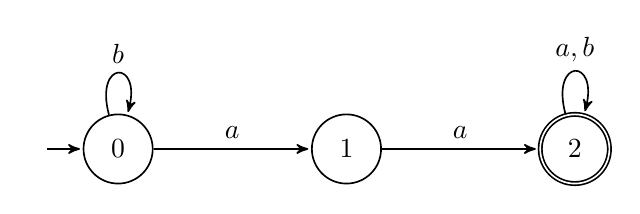
\begin{tikzpicture}[->,>=stealth',shorten >=1pt,auto,node distance=2.9cm,
                    semithick]
  \tikzstyle{every state}=[fill=white,text=black]
  \tikzstyle{place}=[rectangle,draw=black,fill=white, minimum size=7mm]


  \node[initial,state] (A)                    {$0$};
  \node[state] (B)      [right of=A]                {$1$};
  \node[accepting,state] (C)      [right of=B]                {$2$};

  \path %(I) edge[loop above]              node {$a,b$} (I)
(A) edge      [loop above]        node {$b$} (A)
(C) edge      [loop above]        node {$a,b$} (C)
(A) edge      []        node {$a$} (B)
(B) edge      []        node {$a$} (C);
\end{tikzpicture}
\caption{Un automate incomplet}
\label{incompauto}
\end{figure}


\begin{exercice}
Les mots $bbbaababbaaba$, $bbabaab$ et $baaaaaab$ sont-ils acceptés par l'automate de la figure \ref{incompauto} ?
\end{exercice}

\begin{exercice}
Quel est le langage reconnu par l'automate de la figure \ref{incompauto} ? Donner la réponse en français et sous forme d'expression rationnelle.
\end{exercice}


Il nous semble important d'insister sur le point suivant : de la même façon qu'un programme devrait la traduction d'une logique sous-jacente plutôt qu'un bidouaille fait à la va-vite, les états d'un automate ont un sens. Avant d'écrire un automate, il convient donc de réfléchir quelles sont les informations à retenir au cours de la lecture du mot. Si la bonne réponse est trouvée, le reste de l'automate devrait s'écrire seul.

\begin{example}
\label{exemplePI}
On veut écrire un automate reconnaissant le langage $L = \{w \in \Sigma^*~|~|w|_a$ pair et $|w|_b$ impair$\}$, cad. l'ensemble des mots avec un nombre pair de $a$ et impairs de $b$\footnote{On conseillera tout d'abord au lecteur ou à la lectrice de tenter lui/elle-même l'exercice, afin de mesurer la pertinence de l'approche ici présentée}.

Il n'est pas question de compter les $a$ et les $b$ comme on pourrait naïvement l'imaginer, non seulement puisqu'il faut se contenter d'un nombre fini d'états, mais aussi parce que c'est beaucoup plus d'information que nécessaire.
Les seules données qui nous intéressent sont en effet la parité du nombre de $a$ et du nombre de $b$ du mot donné : $a^2b$ comme $a^{26}b^{131}$ sont équivalents dans leur appartenance à $L$.

Le nombre de $a$ et de $b$ étant tous les deux pairs ou impairs, on a 4 possibilités. Nos états s'appeleront $PP$ (nombre de $a$ pair et nombre de $b$ pair), $PI$ ($a$ pair et $b$ impair), $IP$ et $II$. La définition de $L$ nous dit immédiatement que seul $PI$ devrait être terminal. L'état initial devrait être celui qui correspond à $\epsilon$, cad. $PP$.

Les transitions s'écrivent naturellement : en partant de $PP$, la lecture d'un $a$ change la parité du nombre de $a$ mais pas celle du nombre de $b$, et nous emmène donc vers $IP$, tandis que $b$ pointe vers $PI$, et ainsi de suite. S'il y a d'autres lettres dans l'alphabet, elles devraient faire des boucles, puisqu'elles ne changent rien aux parités qui nous intéressent.

Au final, on obtient l'automate suivant : 


\centering
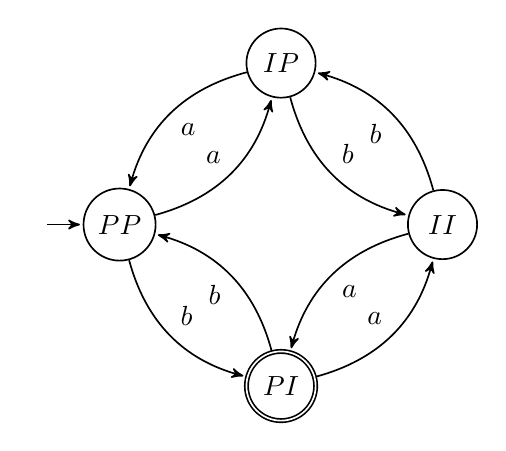
\begin{tikzpicture}[->,>=stealth',shorten >=1pt,auto,node distance=2.9cm,
                    semithick]
  \tikzstyle{every state}=[fill=white,text=black]
  \tikzstyle{place}=[rectangle,draw=black,fill=white, minimum size=7mm]


  \node[initial,state] (PP)                    {$PP$};
  \node[state] (IP)      [above right of=PP]                {$IP$};  \node[state] (II)      [below right of=IP]                {$II$};
  \node[accepting,state] (PI)      [below right of=PP]                {$PI$};

  \path %(I) edge[loop above]              node {$a,b$} (I)
(PP) edge      [bend right]        node {$a$} (IP)
(PP) edge      [bend right]        node {$b$} (PI)
(PI) edge      [bend right]        node {$a$} (II)
(PI) edge      [bend right]        node {$b$} (PP)
(IP) edge      [bend right]        node {$a$} (PP)
(IP) edge      [bend right]        node {$b$} (II)
(II) edge      [bend right]        node {$a$} (PI)
(II) edge      [bend right]        node {$b$} (IP);
\end{tikzpicture}
\end{example}

\begin{exercice} (**) En reprenant l'exemple \ref{exemplePI}, montrer que $\forall w, w \in L \leftrightarrow$ l'automate accepte $w$. Vous pouvez procéder par induction sur $w$, en utilisant un objectif un peu plus précis que celui fourni.
\end{exercice}

%Dans la série d'exercices qui suit, on utilisera comme alphabet $\Sigma = \{a,b\}$.

%\begin{exercice}
%Donner un automate qui reconnaît le langage $\{w \in \Sigma^*~|~|w| \geq 3\}$. 
%\end{exercice}


\subsection{Formalisation}

\section{Automates finis non-déterministes}
\label{NDFA}

\subsection{Principe général}

\subsection{Formalisation}

\section{Transformation d'automates}
\label{transauto}

\subsection{Complétion}

\subsection{Déterminisation}

\subsection{Minimisation}

\section{Propriétés de clôture}
\label{cloture}
\subsection{Union}

\subsection{Intersection}

\subsection{Concaténation}

\subsection{Itération}



\chapter{Théorème de Kleene}
\label{hierarchie}

On a pour l'instant utilisé les expressions rationnelles pour décrire les langages reconnus par des automates, et utilisé des automates pour implémenter des expressions rationnelles. On a cependant vu que l'expressivité des automates était limitée, en ce qu'il existe de nombreux langages qu'ils ne peuvent reconnaître. On peut donc légitimement se demander si les expressions rationnelles sont plus ou moins expressives que les automates finis.

Le mathématicien Stephen C. Kleene (1909 - 1994) répond à cette question via le théorème qui porte son nom :

\begin{theorem}{\textbf{(Théorème de Kleene)}}
Les langages représentable par expression rationnelle sont exactement ceux reconnus par automate fini.
\end{theorem}

L'égalité entre deux ensembles $A$ et $B$ équivaut à la double inclusion entre les mêmes ensembles, cad. $A \subseteq B \wedge B \subseteq A$. On va donc chercher une preuve que chaque langage représentable par \textit{regex} est reconnaissable par automate fini, et inversement. Ces deux sous-théorèmes admettent aujourd'hui de nombreuses preuves, notamment constructives, cad. sous la forme d'algorithmes qui réalisent la transformation d'une \textit{regex} en automate, et inversement. Cette section présente plusieurs de ces algorithmes.

\section{Des expressions rationnelles aux automates}

On veut prouver ici le théorème suivant :

\begin{theorem}
Les langages représentables par expression rationnelle sont également reconnaissables par automate fini.
\end{theorem}

On en présente ici deux preuves différentes.

\subsection{Traduction récursive}

\begin{proof}
On va procéder par induction structurelle sur les expressions rationnelles. On en rappelle d'abord la définition récursive : 

\begin{tabular}{cccl}
$e$ & $\textcolor{black}{::=}$ & & $\epsilon$\\
& & $|$&  $a \in \Sigma$\\
& & $|$&  $e_1.e_2$\\
& & $|$&  $e_1+e_2$\\
& & $|$&  $e_1^*$\\
\end{tabular}

L'expression $\epsilon$ est clairement reconnu par l'automate 


\begin{figure}[H]
\centering
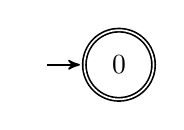
\begin{tikzpicture}[->,>=stealth',shorten >=1pt,auto,node distance=2.9cm,
                    semithick]
  \tikzstyle{every state}=[fill=white,text=black]
  \tikzstyle{place}=[rectangle,draw=black,fill=white, minimum size=7mm]

  \node[initial,state,accepting] (0)                    {$0$};
  
\end{tikzpicture}
\end{figure}

L'expression $a$ quant à elle est reconnue par 


\begin{figure}[H]
\centering
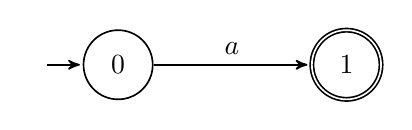
\begin{tikzpicture}[->,>=stealth',shorten >=1pt,auto,node distance=2.9cm,
                    semithick]
  \tikzstyle{every state}=[fill=white,text=black]
  \tikzstyle{place}=[rectangle,draw=black,fill=white, minimum size=7mm]


  \node[initial,state] (0)                    {$0$};
  \node[state,accepting] (1)      [right of=0]                {$1$};

  \path %(I) edge[loop above]              node {$a,b$} (I)
(0) edge      []        node {$a$} (1);

\end{tikzpicture}
\end{figure}

On peut donc traduire en automates les cas de base des expressions rationnelles. Quant aux cas récursifs, on les a en fait déjà traités en \ref{cloture} : pour construire un automate reconnaissant $e_1 + e_2$, on construit des automates $A_1$ et $A_2$ reconnaissant $e_1$ et $e_2$, et on applique la construction de l'union. On procède de même avec la concaténation pour $e_1e_2$ et l'itération pour $e^*$.
\end{proof}

\paragraph*{Remarque} Les constructions vues pour les propriétés de clôture ne sont pas optimales. L'\href{https://fr.wikipedia.org/wiki/Algorithme_de_Thompson}{algorithme de Thomson} utilise les mêmes idées mais s'assure qu'il n'y ait pas plus d'un état initial et un état terminal (différents) tout au long de la construction de l'automate, ce qui permet de borner plus finement sa taille, et de faciliter la concaténation (on fusionne l'état terminal gauche et l'état initial droit).

\subsection{Traduction linéaire}

On propose un autre algorithme, qui sépare la construction des états de celles des transitions : l'\textbf{algorithme de Glushkov}.

\begin{example}

Soit $e = (abb^*a+(ba)^*)^*$. On commence par distinguer toutes les lettres de l'expression, par exemple en les indexant par leur position. On obtient donc

\[
(a_1b_2b_3^*a_4+(b_5a_6)^*)^*
\]

On crée ensuite un état pour chaque lettre, ainsi qu'un état initial $0$ :


\begin{figure}[H]
\centering
\begin{tikzpicture}[->,>=stealth',shorten >=1pt,auto,node distance=2.5cm,
                    semithick]
  \tikzstyle{every state}=[fill=white,text=black]
  \tikzstyle{place}=[rectangle,draw=black,fill=white, minimum size=7mm]

  \node[initial,state] (0)                    {$0$};
  \node[state] (1)   [above right of=0]                {$a_1$};
  \node[state] (2)    [right of=1]     {$b_2$};
  \node[state] (3)             [right of=2]       {$b_3$};
  \node[state] (4)        [right of=3]            {$a_4$};
  \node[state] (5)     [below right of=0]               {$b_5$};
  \node[state] (6)     [right of=5]               {$a_6$};


%  \path %(I) edge[loop above]              node {$a,b$} (I)
%(0) edge      []        node {$a$} (1);

\end{tikzpicture}
\end{figure}

Le jeu va être de représenter, avec les transitions, les "promenades" dans l'expression. Toute mot capturé par l'expression commence par $a_1$ ou $b_5$. On ajoute donc ces transitions : 


\begin{figure}[H]
\centering
\begin{tikzpicture}[->,>=stealth',shorten >=1pt,auto,node distance=2.5cm,
                    semithick]
  \tikzstyle{every state}=[fill=white,text=black]
  \tikzstyle{place}=[rectangle,draw=black,fill=white, minimum size=7mm]

  \node[initial,state] (0)                    {$0$};
  \node[state] (1)   [above right of=0]                {$a_1$};
  \node[state] (2)    [right of=1]     {$b_2$};
  \node[state] (3)             [right of=2]       {$b_3$};
  \node[state] (4)        [right of=3]            {$a_4$};
  \node[state] (5)     [below right of=0]               {$b_5$};
  \node[state] (6)     [right of=5]               {$a_6$};


  \path %(I) edge[loop above]              node {$a,b$} (I)
(0) edge      []        node {$a_1$} (1)
(0) edge      []        node {$b_5$} (5)
;

\end{tikzpicture}
\end{figure}


Quand on a lu un $a_1$, on est obligé de lire un $b_2$. De même, un $b_5$ est forcément suivi d'un $a_6$ :

\begin{figure}[H]
\centering
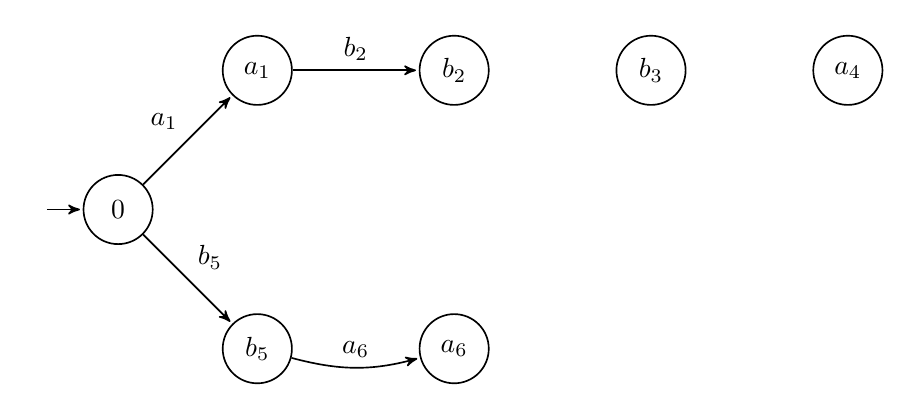
\begin{tikzpicture}[->,>=stealth',shorten >=1pt,auto,node distance=2.5cm,
                    semithick]
  \tikzstyle{every state}=[fill=white,text=black]
  \tikzstyle{place}=[rectangle,draw=black,fill=white, minimum size=7mm]

  \node[initial,state] (0)                    {$0$};
  \node[state] (1)   [above right of=0]                {$a_1$};
  \node[state] (2)    [right of=1]     {$b_2$};
  \node[state] (3)             [right of=2]       {$b_3$};
  \node[state] (4)        [right of=3]            {$a_4$};
  \node[state] (5)     [below right of=0]               {$b_5$};
  \node[state] (6)     [right of=5]               {$a_6$};


  \path %(I) edge[loop above]              node {$a,b$} (I)
(0) edge      []        node {$a_1$} (1)
(0) edge      []        node {$b_5$} (5)
(1) edge      []        node {$b_2$} (2)
(5) edge      [bend right=15]        node {$a_6$} (6)
;

\end{tikzpicture}
\end{figure}

Après la lecture d'un $a_6$, on peut recommencer la boucle $(b_5a_6)^*$, auquel cas on lit un $b_5$, ou recommencer la boucle entière $(a_1b_2b_3^*a_4+(b_5a_6)^*)^*$, en lisant un $a_1$ ou un $b_5$ :


\begin{figure}[H]
\centering
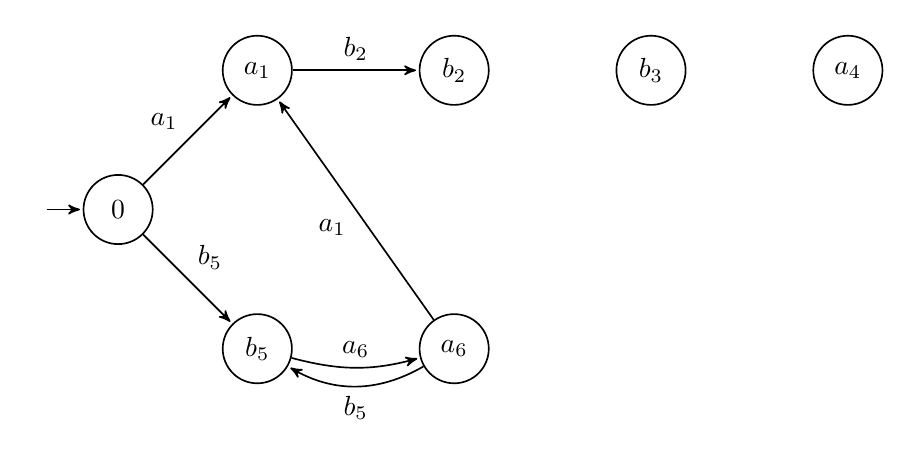
\begin{tikzpicture}[->,>=stealth',shorten >=1pt,auto,node distance=2.5cm,
                    semithick]
  \tikzstyle{every state}=[fill=white,text=black]
  \tikzstyle{place}=[rectangle,draw=black,fill=white, minimum size=7mm]

  \node[initial,state] (0)                    {$0$};
  \node[state] (1)   [above right of=0]                {$a_1$};
  \node[state] (2)    [right of=1]     {$b_2$};
  \node[state] (3)             [right of=2]       {$b_3$};
  \node[state] (4)        [right of=3]            {$a_4$};
  \node[state] (5)     [below right of=0]               {$b_5$};
  \node[state] (6)     [right of=5]               {$a_6$};


  \path %(I) edge[loop above]              node {$a,b$} (I)
(0) edge      []        node {$a_1$} (1)
(0) edge      []        node {$b_5$} (5)
(1) edge      []        node {$b_2$} (2)
(5) edge      [bend right=15]        node {$a_6$} (6)
(6) edge      [bend left]        node {$b_5$} (5)
(6) edge      []        node {$a_1$} (1)
;

\end{tikzpicture}
\end{figure}

Après la lecture d'un $b_2$, on peut lire un $b_3$, mais aussi sauter $b_3^*$ et aller directement lire un $a_4$. En $b_3$, on peut boucler ou passer en $a_4$. En $a_4$, comme en $a_6$, on peut lire $a_1$ ou $b_5$. On a donc :

\begin{figure}[H]
\centering
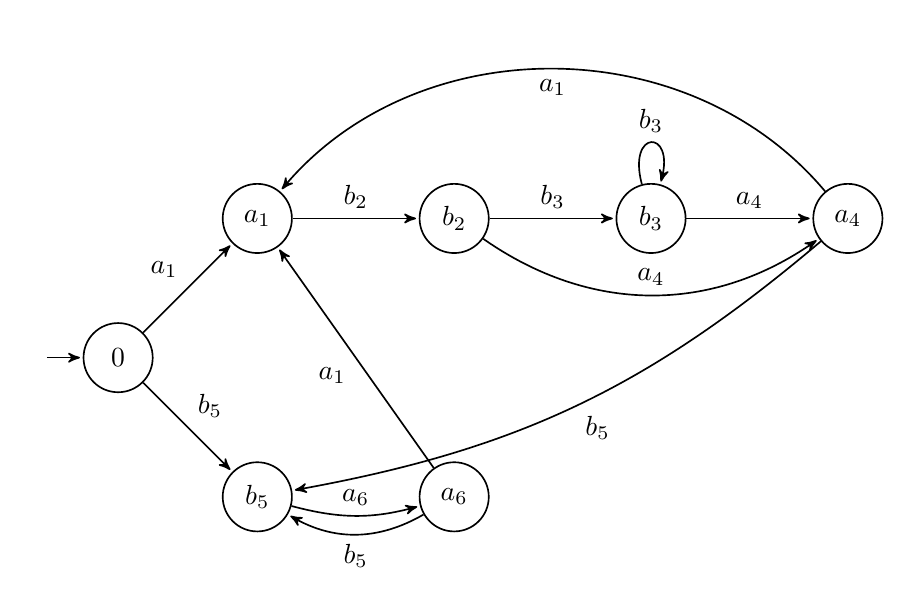
\begin{tikzpicture}[->,>=stealth',shorten >=1pt,auto,node distance=2.5cm,
                    semithick]
  \tikzstyle{every state}=[fill=white,text=black]
  \tikzstyle{place}=[rectangle,draw=black,fill=white, minimum size=7mm]

  \node[initial,state] (0)                    {$0$};
  \node[state] (1)   [above right of=0]                {$a_1$};
  \node[state] (2)    [right of=1]     {$b_2$};
  \node[state] (3)             [right of=2]       {$b_3$};
  \node[state] (4)        [right of=3]            {$a_4$};
  \node[state] (5)     [below right of=0]               {$b_5$};
  \node[state] (6)     [right of=5]               {$a_6$};


  \path %(I) edge[loop above]              node {$a,b$} (I)
(0) edge      []        node {$a_1$} (1)
(0) edge      []        node {$b_5$} (5)
(1) edge      []        node {$b_2$} (2)
(2) edge      []        node {$b_3$} (3)
(2) edge      [bend right=35]        node {$a_4$} (4)
(3) edge      []        node {$a_4$} (4)
(3) edge      [loop above]        node {$b_3$} (3)
(4) edge      [bend right=50]        node {$a_1$} (1)
(4) edge      [bend left=15]        node {$b_5$} (5)
(5) edge      [bend right=15]        node {$a_6$} (6)
(6) edge      [bend left]        node {$b_5$} (5)
(6) edge      []        node {$a_1$} (1)
;

\end{tikzpicture}
\end{figure}

On peut arrêter de boucler quand on vient de lire un $a_4$ ou un $a_6$, ce qui veut dire que les états correspondant vont être terminaux. De plus, l'expression rationnelle contient le mot vide, ce qui veut dire que l'état initial doit être terminal. Il ne nous reste plus qu'à "déspécialiser" les lettres, et éventuellement renommer les états :


\begin{figure}[H]
\centering
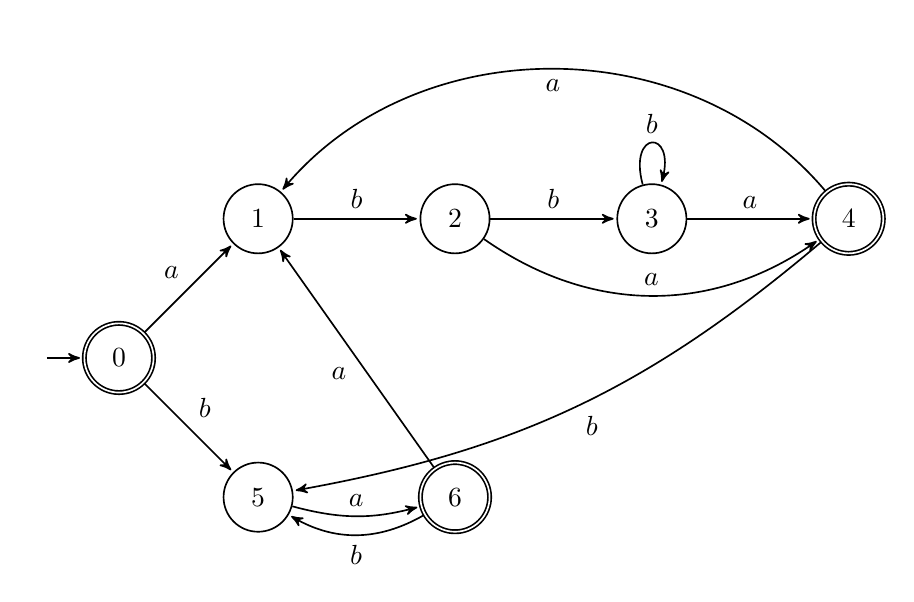
\begin{tikzpicture}[->,>=stealth',shorten >=1pt,auto,node distance=2.5cm,
                    semithick]
  \tikzstyle{every state}=[fill=white,text=black]
  \tikzstyle{place}=[rectangle,draw=black,fill=white, minimum size=7mm]

  \node[initial,state,accepting] (0)                    {$0$};
  \node[state] (1)   [above right of=0]                {$1$};
  \node[state] (2)    [right of=1]     {$2$};
  \node[state] (3)             [right of=2]       {$3$};
  \node[state,accepting] (4)        [right of=3]            {$4$};
  \node[state] (5)     [below right of=0]               {$5$};
  \node[state,accepting] (6)     [right of=5]               {$6$};


  \path %(I) edge[loop above]              node {$a,b$} (I)
(0) edge      []        node {$a$} (1)
(0) edge      []        node {$b$} (5)
(1) edge      []        node {$b$} (2)
(2) edge      []        node {$b$} (3)
(2) edge      [bend right=35]        node {$a$} (4)
(3) edge      []        node {$a$} (4)
(3) edge      [loop above]        node {$b$} (3)
(4) edge      [bend right=50]        node {$a$} (1)
(4) edge      [bend left=15]        node {$b$} (5)
(5) edge      [bend right=15]        node {$a$} (6)
(6) edge      [bend left]        node {$b$} (5)
(6) edge      []        node {$a$} (1)
;

\end{tikzpicture}
\end{figure}
\end{example}

On a présenté l'algorithme \textit{via} un exemple, mais il repose bien évidemment sur des définitions formelles, procédant par induction sur l'expression. Une fois qu'on a spécialisé les lettres et crée les états comme dans l'exemple, on veut d'abord savoir si l'expression rationnelle donnée accepte ou non le mot vide. C'est à cette question que répond la fonction suivante :

\[
\begin{cases}
E(\epsilon) = \top \\
E(a) = \bot \\
E(e_1+e_2) = E(e_1) \vee E(e_2) \\
E(e_1.e_2) = E(e_1) \wedge E(e_2) \\
E(e^*) = \top
\end{cases}
\]

L'état initial est terminal ssi. $E(e) = \top$. Pour les premières transitions, qui partiront de l'état initial $0$, on a besoin de déterminer quelles lettres peuvent commencer les mots reconnus par l'expression, ce que fait la fonction suivante : 

\[
\begin{cases}
D(\epsilon) = \emptyset \\
D(a) = \{a\} \\
D(e_1+e_2) = D(e_1) \cup D(e_2) \\
D(e_1.e_2) = D(e_1) & \text{Si } e_1 \text{ n'accepte pas le mot vide, cad. si }\neg E(e_1)\\
D(e_1.e_2) = D(e_1) \cup D(e_2) & \text{sinon}  \\
D(e^*) = D(e)
\end{cases}
\]

On ajoute une transition $0 \xrightarrow{q} q$ pour tout $q \in D(e)$. De même, on a besoin de savoir quelles lettres peuvent finir les mots du langage dénoté par une expression : 

\[
\begin{cases}
F(\epsilon) = \emptyset \\
F(a) = \{a\} \\
F(e_1+e_2) = F(e_1) \cup F(e_2) \\
F(e_1.e_2) = F(e_2) & \text{Si } e_2 \text{ n'accepte pas le mot vide, cad. si} \neg E(e_2)\\f
F(e_1.e_2) = F(e_1) \cup F(e_2) & \text{sinon}  \\
F(e^*) = F(e)
\end{cases}
\]


Tout les états de $F$ sont terminaux. En plus des premières transitions, on veut bien sûr les autres. Pour ça, on calcule l'ensemble des lettres qui peuvent se suivre dans le langage dénoté par l'expression :

\[
\begin{cases}
P(\epsilon) = \emptyset \\
P(a) = \emptyset \\
P(e_1+e_2) = P(e_1) \cup P(e_2) \\
P(e_1.e_2) = P(e_1) \cup P(e_2) \cup F(e_1).D(e_2) \\
P(e^*) = P(e) \cup F(e).D(e) 
\end{cases}
\]

Toute paire $\big \langle q_1, q_2 \big \rangle$ appartenant à $P(e)$ génère donc une transition $q_1 \xrightarrow{q_2} q_2$ dans l'automate.


\begin{exercice}
Utiliser l'algorithme de Glushkov pour traduire en automate l'expression \newline $e = (bb)^*(b(a+b)^*)^*$
\end{exercice}

\paragraph*{Remarque} On a présenté ces différents algorithmes comme des preuves de la "traductabilité" des expressions rationnelles en automates finis. Si on était vraiment rigoureux, les algorithmes ne suffiraient pas, il faudrait aussi prouver 1) qu'ils terminent sur toute entrée 2) qu'ils produisent bien un automate fini acceptant le langage décrit par l'expression donnée. Ces preuves sont autrement plus complexes que l'écriture des algorithmes\footnote{On entend souvent dire que la preuve d'un programme ou algorithme est au moins un ordre de grandeur plus complexe que l'écriture de ce dernier} et vont au-delà du programme du cours, mais il est toujours bon de garder son esprit critique face à ces choses. Cette remarque s'applique bien évidemment également à l'algorithme présenté dans les pages qui suivent pour la traduction inverse.



\section{Des automates aux expressions rationnelles - algorithme de McNaughton et Yamada}

On veut maintenant prouver le théorème suivant :

\begin{theorem}
Les langages reconnaissables par automate fini sont représentables par expression rationnelle.
\end{theorem}

On en présente ici une preuve constructive, connue sous le nom d'algorithme de McNaughton et Yamada.

\begin{proof}
Soit un automate $A$ ayant comme ensemble d'états $Q$. L'idée va être de calculer, pour toute paire d'états $(i,j)$, les ensembles de mots permettant d'aller de $i$ à $j$ en n'utilisant qu'une sélection d'états. On va faire ces calculs pour des sélections minimales, et grossir petit à petit, jusqu'à ne plus avoir de contrainte. 


On introduit pour ça la notation $L_{i,j}^X$, qui représente sous forme d'expression rationnelle l'ensemble des mots \underline{non-vides} menant de $i$ à $j$ en n'utilisant \underline{comme états intermédiaires} que des états appartenant à l'ensemble $X$. Par exemple, dans l'automate  

\begin{figure}[H]
\centering
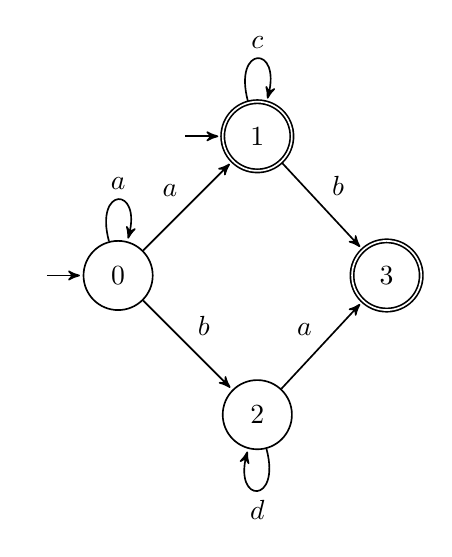
\begin{tikzpicture}[->,>=stealth',shorten >=1pt,auto,node distance=2.5cm,
                    semithick]
  \tikzstyle{every state}=[fill=white,text=black]
  \tikzstyle{place}=[rectangle,draw=black,fill=white, minimum size=7mm]

  \node[initial,state] (0)                    {$0$};
  \node[initial,state,accepting] (1)   [above right of=0]                {$1$};
  \node[state] (2)    [below right of=0]     {$2$};
  \node[state,accepting] (3)             [right=2.5cm of 0]       {$3$};


  \path %(I) edge[loop above]              node {$a,b$} (I)
(0) edge      [loop above]        node {$a$} (0)
(1) edge      [loop above]        node {$c$} (1)
(2) edge      [loop below]        node {$d$} (2)
(0) edge      []        node {$a$} (1)
(0) edge      []        node {$b$} (2)
(1) edge      []        node {$b$} (3)
(2) edge      []        node {$a$} (3)
;

\end{tikzpicture}
\end{figure}

$L_{0,3}^{\{1\}} = ac^*b$. En effet, on ne peut pas boucler en $0$ car il servirait alors d'état intermédiaire, alors qu'il ne fait pas partie de ceux autorisés. De même, on ne peut pas passer par l'état $2$. On peut en revanche boucler sur $1$, d'où le $c^*$ dans la regex.

On commence en calculer tous les $L_{i,j}^{\emptyset}$. Puisqu'on n'a pas le droit au moindre état intermédiaire, $L_{i,j}^{\emptyset}$ vaut la lettre étiquettant la transition de $i$ à $j$ si elle existe, et $\emptyset$ sinon. Dans notre exemple, on a donc 

\begin{itemize}
\item En partant de $0$ :
   \begin{itemize}
	 \item $L_{0,0}^{\emptyset} = a$
	 \item $L_{0,1}^{\emptyset} = a$
	 \item $L_{0,2}^{\emptyset} = b$
	 \item $L_{0,3}^{\emptyset} = \emptyset$
   \end{itemize}
\item En partant de $1$ :
   \begin{itemize}
	 \item $L_{1,0}^{\emptyset} = \emptyset$
	 \item $L_{1,1}^{\emptyset} = c$
	 \item $L_{1,2}^{\emptyset} = \emptyset$
	 \item $L_{1,3}^{\emptyset} = b$
   \end{itemize}
\item En partant de $2$ :
   \begin{itemize}
	 \item $L_{2,0}^{\emptyset} = \emptyset$
	 \item $L_{2,1}^{\emptyset} = \emptyset$
	 \item $L_{2,2}^{\emptyset} = d$
	 \item $L_{2,3}^{\emptyset} = a$
   \end{itemize}
\item En partant de $3$ :
   \begin{itemize}
	 \item $L_{3,0}^{\emptyset} = \emptyset$
	 \item $L_{3,1}^{\emptyset} = \emptyset$
	 \item $L_{3,2}^{\emptyset} = \emptyset$
	 \item $L_{3,3}^{\emptyset} = \emptyset$
   \end{itemize}
\end{itemize}

Maintenant qu'on a notre cas de base, il s'agit de passer aux étapes suivantes en ajoutant de nouveaux états. Si on a tous nos $L_{i,j}^X$ et qu'on veut s'autoriser à passer par l'état $q$, on va utiliser la formule 

\[
L_{i,j}^{X \cup \{q\}} = L_{i,j}^X \cup L_{i,q}^X(L_{q,q}^X)^*L_{q,j}^X
\]

L'idée est que, pour aller de $i$ à $j$ en ayant le droit d'utiliser les états de $X$ et $q$, on passe ou non par $q$. Le deuxième cas est pris en compte la partie gauche de l'union ensembliste.

Supposons maintenant qu'on aille de $i$ à $j$ en passant au moins une fois par $q$. Dans ce cas, notre parcours commence par un chemin de $i$ à $q$ sans passer par $q$, cad. par la lecture d'un mot appartenant à $L_{i,q}^X$.

Le parcours peut passer plus d'une fois par $q$. On s'autoriste donc à faire des chemins de $q$ à $q$, ce qui correspond à la partie $(L_{q,q}^X)^*$ de la formule.

Enfin, une fois qu'on a fait notre dernier passage par l'état $q$, il faut finir notre parcours en allant en $j$ : $L_{q,j}^X$.

En résumé, pour calculer l'ensemble des mots menant de $i$ à $j$ en passant par les états de $X$ ou $q$, on isole explicitement les éventuels passages par $q$ pour pouvoir se ramener au cas précédent, où seuls les états appartenant à $X$ sont autorisés. On peut donc maintenant avancer les calculs pour notre automate, par exemple en autorisant maintenant les passages par l'état $1$ (l'ordre dans lequel on ajoute les états ne change pas le résultat, mais peut rendre les calculs plus ou moins longs) :


\begin{itemize}
\item En partant de $0$ :
   \begin{itemize}
	 \item $L_{0,0}^{\emptyset \cup \{1\}} = L_{0,0}^{\emptyset} \cup L_{0,1}^{\emptyset}(L_{1,1}^{\emptyset})^*L_{1,0}^{\emptyset} = a + a(c)^*\emptyset = a$\footnote{Pour rappel, $L\emptyset = \emptyset L = \emptyset$ pour tout langage $L$}
	 \item $L_{0,1}^{\{1\}} = L_{0,1}^{\emptyset} \cup L_{0,1}^{\emptyset}(L_{1,1}^{\emptyset})^*L_{1,1}^{\emptyset} = a + ac^*c = a + ac^+ = ac^*$
	 \item $L_{0,2}^{\{1\}} = L_{0,2}^{\emptyset} \cup L_{0,1}^{\emptyset}(L_{1,1}^{\emptyset})^*L_{1,2}^{\emptyset} = b + ac^*\emptyset = b$
	 \item $L_{0,3}^{\{1\}} = L_{0,3}^{\emptyset} \cup L_{0,1}^{\emptyset}(L_{1,1}^{\emptyset})^*L_{1,3}^{\emptyset} = ac^*b$
   \end{itemize}
\item En partant de $1$ :
   \begin{itemize}
	 \item $L_{1,0}^{\{1\}} = L_{1,0}^{\emptyset} \cup L_{1,1}^{\emptyset}(L_{1,1}^{\emptyset})^*L_{1,0}^{\emptyset} = \emptyset$
	 \item $L_{1,1}^{\{1\}} = L_{1,1}^{\emptyset} \cup L_{1,1}^{\emptyset}(L_{1,1}^{\emptyset})^*L_{1,1}^{\emptyset} = c + cc^*c = c^+$
	 \item $L_{1,2}^{\{1\}} = L_{1,2}^{\emptyset} \cup L_{1,1}^{\emptyset}(L_{1,1}^{\emptyset})^*L_{1,2}^{\emptyset} = \emptyset$
	 \item $L_{1,3}^{\{1\}} = L_{1,3}^{\emptyset} \cup L_{1,1}^{\emptyset}(L_{1,1}^{\emptyset})^*L_{1,3}^{\emptyset} = b + cc^*b = b + c^+b = c^*b$
   \end{itemize}
\item En partant de $2$ :
   \begin{itemize}
	 \item $L_{2,0}^{\{1\}} = L_{2,0}^{\emptyset} \cup L_{2,1}^{\emptyset}(L_{1,1}^{\emptyset})^*L_{1,0}^{\emptyset} = \emptyset$
	 \item $L_{2,1}^{\{1\}} = L_{2,1}^{\emptyset} \cup L_{2,1}^{\emptyset}(L_{1,1}^{\emptyset})^*L_{1,1}^{\emptyset} = \emptyset$
	 \item $L_{2,2}^{\{1\}} = L_{2,2}^{\emptyset} \cup L_{2,1}^{\emptyset}(L_{1,1}^{\emptyset})^*L_{1,2}^{\emptyset} = d$
	 \item $L_{2,3}^{\{1\}} = L_{2,3}^{\emptyset} \cup L_{2,1}^{\emptyset}(L_{1,1}^{\emptyset})^*L_{1,3}^{\emptyset} = a$
   \end{itemize}
\item En partant de $3$, vu que $L_{3,j}^{\emptyset} = \emptyset$ pour tout état $j$, on n'arrivera jamais à aller plus loin. Donc $L_{3,j}^{\{1\}} = \emptyset$ pour tout $j$.
\end{itemize}

On continue en ajoutant $2$ : 


\begin{itemize}
\item En partant de $0$ :
   \begin{itemize}
	 \item $L_{0,0}^{\{1\} \cup \{2\}} = L_{0,0}^{\{1\}} \cup L_{0,2}^{\{1\}}(L_{2,2}^{\{1\}})^*L_{2,0}^{\{1\}} = a$
	 \item $L_{0,1}^{\{1,2\}} = L_{0,1}^{\{1\}} \cup L_{0,2}^{\{1\}}(L_{2,2}^{\{1\}})^*L_{2,1}^{\{1\}} = ac^*$
	 \item $L_{0,2}^{\{1,2\}} = L_{0,2}^{\{1\}} \cup L_{0,2}^{\{1\}}(L_{2,2}^{\{1\}})^*L_{2,2}^{\{1\}} = b + bd^*d = bd^*$
	 \item $L_{0,3}^{\{1,2\}} = L_{0,3}^{\{1\}} \cup L_{0,2}^{\{1\}}(L_{2,2}^{\{1\}})^*L_{2,3}^{\{1\}} = ac^*b + bd^*a$
   \end{itemize}
\item En partant de $1$ :
   \begin{itemize}
	 \item $L_{1,0}^{\{1,2\}} = L_{1,0}^{\{1\}} \cup L_{1,2}^{\{1\}}(L_{2,2}^{\{1\}})^*L_{2,0}^{\{1\}} = \emptyset$
	 \item $L_{1,1}^{\{1,2\}} = L_{1,1}^{\{1\}} \cup L_{1,2}^{\{1\}}(L_{2,2}^{\{1\}})^*L_{2,1}^{\{1\}} = c^+$
	 \item $L_{1,2}^{\{1,2\}} = L_{1,2}^{\{1\}} \cup L_{1,2}^{\{1\}}(L_{2,2}^{\{1\}})^*L_{2,2}^{\{1\}} = \emptyset$
	 \item $L_{1,3}^{\{1,2\}} = L_{1,3}^{\{1\}} \cup L_{1,2}^{\{1\}}(L_{2,2}^{\{1\}})^*L_{2,3}^{\{1\}} = c^*b$
   \end{itemize}
\item En partant de $2$ :
   \begin{itemize}
	 \item $L_{2,0}^{\{1,2\}} = L_{2,0}^{\{1\}} \cup L_{2,2}^{\{1\}}(L_{2,2}^{\{1\}})^*L_{2,0}^{\{1\}} = \emptyset$
	 \item $L_{2,1}^{\{1,2\}} = L_{2,1}^{\{1\}} \cup L_{2,2}^{\{1\}}(L_{2,2}^{\{1\}})^*L_{2,1}^{\{1\}} = \emptyset$
	 \item $L_{2,2}^{\{1,2\}} = L_{2,2}^{\{1\}} \cup L_{2,2}^{\{1\}}(L_{2,2}^{\{1\}})^*L_{2,2}^{\{1\}} = d + dd^*d = d^+$
	 \item $L_{2,3}^{\{1,2\}} = L_{2,3}^{\{1\}} \cup L_{2,2}^{\{1\}}(L_{2,2}^{\{1\}})^*L_{2,3}^{\{1\}} = a + dd^*a = d^*a$
   \end{itemize}
\item $L_{3,j}^{\{1,2\}} = \emptyset$ pour tout $j$.
\end{itemize}

On ajoute maintenant $0$ : 


\begin{itemize}
\item En partant de $0$ :
   \begin{itemize}
	 \item $L_{0,0}^{\{1,2\} \cup \{0\}} = L_{0,0}^{\{1,2\}} \cup L_{0,0}^{\{1,2\}}(L_{0,0}^{\{0,2\}})^*L_{0,0}^{\{1,2\}} = a + aa^*a = a^+$
	 \item $L_{0,1}^{\{0,1,2\}} = L_{0,1}^{\{1,2\}} \cup L_{0,0}^{\{1,2\}}(L_{0,0}^{\{1,2\}})^*L_{0,1}^{\{1,2\}} = ac^* + aa^*ac^* = a^+c^*$
	 \item $L_{0,2}^{\{0,1,2\}} = L_{0,2}^{\{1,2\}} \cup L_{0,0}^{\{1,2\}}(L_{0,0}^{\{1,2\}})^*L_{0,2}^{\{1,2\}} = bd^* + aa^*bd^* = a^*bd^*$
	 \item $L_{0,3}^{\{0,1,2\}} = L_{0,3}^{\{1,2\}} \cup L_{0,0}^{\{1,2\}}(L_{0,0}^{\{1,2\}})^*L_{0,3}^{\{1,2\}} = ac^*b + bd^*a + aa^*(ac^*b + bd^*a) = a^*(ac^*b + bd^*a)$
   \end{itemize}
\item Comme on en a un peu marre, on remarque que $L_{i,0}^{\{1,2\}} = \emptyset$ quand $i \neq 0$, et donc que $L_{i,0}^{\{1,2\}}(L_{0,0}^{\{1,2\}})^*L_{0,j}^{\{1,2\}} = \emptyset$ pour tout état $j$. Donc, pour les départs d'états autres que $0$, le fait de pouvoir passer par $0$ ne va rien pouvoir ajouter. On a donc $L_{i,0}^{\{0,1,2\}} = L_{i,0}^{\{1,2\}}$ pour $i \neq 0$.
\end{itemize}

De même, $L_{3,i}^{\{0,1,2\}} = \emptyset$ pour tout état $i$. On a donc $L_{i,j}^Q = L_{i,j}^{\{0,1,2\}}$ pour toute paire d'états $i$ et $j$. 


Maintenant qu'on a calculé les langages reconnus par toute paire d'états, on combine ceux qui nous intéressent. Puisque les états initiaux sont $0$ et $1$ et que les terminaux sont $1$ et $3$, le langage reconnu par l'automate est l'union des mots allant de $0$ à $1$, de $0$ à $3$, de $1$ à $1$ et de $1$ à $3$ (on fait toues les combinaisons d'état initial / état terminal).

Attention cependant, $L_{i,j}^Q$ calcule l'ensemble des mots \underline{non-vides} allant de $i$ à $j$. Donc si un état est à la fois initial et terminal, il faut ajouter à la main le mot vide.

En conclusion, le langage reconnu par l'automate de l'exemple est décrit par la regex 

\[
L_{0,1}^Q + L_{0,3}^Q + L_{1,1}^Q + L_{1,3}^Q + \epsilon = a^+c^* + a^*(ac^*b + bd^*a) + c^+ + c^*b + \epsilon
\]

\end{proof}

Etant donné un automate fini, l'algorithme de McNaughton et Yamada permet donc, bien que parfois quelque peu laborieusement, de produire une expression rationnelle décrivant le même langage, réalisant donc la deuxième partie du théorème de Kleene.

\chapter{Grammaires formelles et hiérarchie de Chomsky}
\label{grammaires}


\section{Principe général}

Une \textbf{grammaire formelle} est une série de \textbf{règles} permettant de générer des mots. Ces règles utilisent des \textbf{symboles} dits \textbf{terminaux} (les lettres "normales", par convention en minuscules), et d'autres dits \textbf{non-terminaux} (normalement dénotés par des lettres majuscules). Un de ces symboles non-terminaux, appelé \textbf{axiome}, indique le début de toute génération de mot. On présente d'abord le fonctionnement des grammaires et les concepts de base à l'aide de quelques exemples. 

\begin{example}
On présente la grammaire dénotée par ces deux règles :

\[
\begin{cases}
S \rightarrow \epsilon \\
S \rightarrow abS 
\end{cases}
\]

Cette grammaire contient un seul symbole non-terminal, S. Il s'agit donc automatiquement de l'axiome. Le symbole S peut se transformer en $\epsilon$ (première règle) ou en $abS$ (deuxième règle). Cette grammaire génère l'ensemble des mots composés uniquement de symboles terminaux ($a$ et $b$) qu'on peut obtenir en partant de l'axiome S et en appliquant autant de fois qu'on veut les règles données. Dans ce qui suit, on écrira $\rightarrow_1$ pour une application de la première règle et $\rightarrow_2$ pour la seconde.

On peut par exemple obtenir le mot $ab$ de la façon suivante :

\[
S \rightarrow_2 abS \rightarrow_1 ab
\]

Dans cette suite de transformation, appelée \textbf{dérivation}, on remplace d'abord l'axiome par $abS$ à l'aide de la deuxième règle. Puisque $abS$ contient le facteur $S$, on peut utiliser \textit{localement} la deuxième règle pour faire disparaître ce S. Dans ce cas, ce qu'il y avait autour du S, le \textbf{contexte}, reste inchangé.

On peut également obtenir le mot $abab$ :

\[
S \rightarrow_2 \textcolor{blue}{ab}S \rightarrow_2 \textcolor{blue}{ab}\textcolor{red}{ab}S \rightarrow_1 \textcolor{blue}{ab}\textcolor{red}{ab}
\]

ou ababab :


\[
S \rightarrow_2 \textcolor{blue}{ab}S \rightarrow_2 \textcolor{blue}{ab}\textcolor{red}{ab}S \rightarrow_2 \textcolor{blue}{ab}\textcolor{red}{ab}\textcolor{green}{ab}S \rightarrow_1  \textcolor{blue}{ab}\textcolor{red}{ab}\textcolor{green}{ab}
\]

Il n'est pas obligatoire d'utiliser toutes les règles d'une grammaire. On peut donc générer le mot vide :

\[
S \rightarrow_1 \epsilon
\]

On se rend compte assez vite que la grammaire \textbf{engendre} le langage $(ab)^*$.

\end{example}


%
\chapter{Notion(s) de calculabilité}

Les automates forment un langage de programmation, et donc une façon de penser et d'automatiser le calcul. On commence par introduire deux autres modèles bien connus, puis on discutera du contexte historique et scientifique ayant mené à ces notions.

Ce chapitre ne se substitue pas à une authentique introduction à la calculabilité, et devrait d'ailleurs au strict minimum être complété par \href{https://www.college-de-france.fr/site/xavier-leroy/inaugural-lecture-2018-11-15-18h00.htm}{la magnifique leçon inaugurale de Xavier Leroy au Collège de France}. Il est très probable qu'il contienne des inexactitudes historiques, voire scientifiques. Plutôt que la précision ou l'exhaustivité, il a avant tout pour objectif de contextualiser ceux qui le précèdent, ainsi que de donner une idée, et pourquoi pas le goût, des questions qui se posent dans l'étude des modèles de calcul, ou \textbf{calculabilité}.

\section{Différents modèles de calcul}

L'informatique a pour vocation automatiser ce qui peut l'être afin de faire réaliser ces tâches par des machines plutôt que des humains. Une tâche est automatisable si elle peut être résolue par une série d'instructions sans ambiguïté, c'est-à-dire si elle peut être réduite à des calculs qu'il s'agit de définir formellement. 

D'un point de vue programmation, 2 principaux modèles historiques co-existent : les \textbf{machines de Turing} et le \textbf{$\lambda$-calcul}. Ces langages, qui remontent tout de même aux années 30, ne sont pas utilisables en pratique (\href{http://www.ens-lyon.fr/actualite/lecole/la-machine-de-turing-en-legos}{encore que}), mais posent les fondamentaux de ce qu'est un langage de programmation.

\paragraph{Machines de Turing} Les machines de Turing disposent de la même notion d'état que les automates, mais aussi d'une mémoire infinie modifiable. Cette mémoire, généralement appelée ruban, contient initialement le mot donné en entrée. Comme les automates, les transitions des machines de Turing sont déterminées par l'état actuel ainsi que la lettre lue. Cependant, en plus de potentiellement changer l'état, les transitions indiquent comment se déplacer dans le mot (droite comme dans les automate, mais aussi aller à gauche ou rester sur place) et une éventuelle réécriture. Les machines de Turing peuvent donc manipuler à loisir leur mémoire, quitte à réécrire le mot donné en entrée ou déborder d'un côté ou de l'autre. Cette manipulation explicite de la mémoire, ainsi que le fait qu'elles favorisent l'utilisation de boucles, rapprochent fortement les machines de Turing de la programmation impérative (C, langage machine, le coeur de Python etc). Elles ont été conçues par l'anglais \textbf{Alan Turing}.

\paragraph{$\lambda$-calcul} A la différence des machines de Turing, qui ont une approche quasiment mécanique (pour ne pas dire "bidouille") de l'exécution d'un programme, le $\lambda$-calcul est profondément mathématique et repose sur la récursion. Tout n'y est que fonction, au point que ces dernières sont des objets comme les autres, notamment passables en arguments. On citera l'exemple classique d'une fonction qui reçoit une fonction de tri et une liste, et renvoie la liste triée selon la fonction fournie. Le $\lambda$-calcul est la base de la programmation fonctionnelle. Il a été crée par \textbf{Alonzo Church}.

\paragraph{Remarque} Les types en programmation impérative n'ont souvent qu'une valeur de garde-fou contre des opérations totalement absurdes, alors qu'ils ont une fonction beaucoup plus structurante (certain.e.s diraient "contraignante") en programmation fonctionnelle. L'utilisation de fonctions comme arguments oblige par exemple à repenser les types et aller plus loin que les classiques \verb!bool!, \verb!int! et cie. On renverra encore une fois à la présentation de Xavier Leroy citée en introduction pour une meilleur vision d'ensemble.

Ces deux modèles ne forment pas l'alpha et l'omega de la calculabilité, qui contient de nombreux modèles plus ou moins exotiques, comme les fonctions $\mu$-récursives ou les automates cellulaires (voir à ce sujet \href{https://www.youtube.com/watch?v=S-W0NX97DB0}{la très chouette vidéo de la chaîne ScienceEtonnante}).

\section{Un peu d'Histoire : le programme de Hilbert} 

Bien que développés en isolation, ces deux modèles s'inscrivent dans un même mouvement intellectuel. A l'aube du $20^{eme}$ siècle, les fondements des mathématiques sont mis à mal (pour ne pas dire balayés) par \href{https://en.wikipedia.org/wiki/Foundations_of_mathematics#Foundational_crisis}{plusieurs paradoxes}, dont le plus connu est le paradoxe de Russel. Le mathématicien allemand David Hilbert pose alors les bases d'un grand plan de (re)fondation des mathématiques, aujourd'hui appelé "programme de Hilbert". L'idée était d'obtenir une formalisation de l'intégralité des mathématiques, formalisation qui se devait d'être \textbf{complète}, \textbf{cohérente} et \textbf{décidable}.

\subsection{Complétude et cohérence}
Un système mathématique est dit \textbf{complet} s'il existe un système de règles précis dans lequel tout énoncé qui y est vrai peut être démontré. Par exemple, la logique du premier ordre admet plusieurs systèmes de preuve (déduction naturelle, calcul des séquents, ...), contenant des règles du type "De $A \wedge B$ on peut déduire $A$" ou "Si on a un prédicat $P(x)$ et une constante $a$ telle que $P(a)$ est vrai, alors on peut déduire $\exists x, P(x)$". Le mathématicien austro-hongrois Kurt Gödel montre en 1929 que la logique du premier ordre est complète. 

Il existe donc un système de déduction entièrement formalisé et syntaxique dans lequel on peut démontrer tout énoncé vrai de logique du premier ordre (par exemple $(\exists y, \forall x, P(x,y)) \rightarrow \forall x, \exists y, P(x,y)$). En ce sens, le \textbf{théorème de complétude de Gödel} relie la sémantique (la vérité ou non) et la syntaxe (la déduction par application de règles) de la logique du premier ordre.

Ce résultat, avec d'autres, va dans le sens de Hilbert. La logique du premier ordre est cependant trop faible pour exprimer l'arithmétique, qui constitue à l'époque le graal des mathématiques. Cette réalité sera douloureusement rappelée l'année suivante, en 1930, par Gödel, lorsqu'il présentera son \textit{magnum opus}, appelé aujourd'hui \textbf{théorème d'incomplétude de Gödel}. Ce théorème établit que n'\underline{importe quel système formel} assez puissant pour exprimer les nombres entiers sera incomplet. Quelle que soit la formalisation de l'arithmétique choisie, il y aura donc toujours au moins un résultat vrai qui n'y sera pas prouvable. La preuve de Gödel est très bien vulgarisée dans \href{https://www.youtube.com/watch?v=82jOF4Q6gBU}{cette vidéo}.

Un système mathématique est dit \textbf{cohérent} si on ne peut pas y prouver une chose et son contraire (ou, de façon équivalente, si on ne peut y prouver l'énoncé "faux"). Sans aller jusqu'à casser la cohérence de quel que système mathématique que ce soit, la preuve du théorème d'incomplètude de Gödel a pour corollaire que toute formalisation de l'arithmétique sera incapable de prouver sa propre cohérence - ce qui ne veut pas dire qu'elle ne l'est pas.

Les travaux de Gödel n'enterrent pas le programme de Hilbert, mais lui portent un sacré coup. Il faut en effet revoir à la baisse les ambitions, et arrêter d'espérer une formalisation "absolue" des mathématiques. Dans une de ces cruelles ironies dont l'Histoire a le secret, Gödel a présenté ses travaux lors d'une conférence organisée pour le départ en retraite d'Hilbert.

\subsection{Décidabilité et thèse de Church} 

Au $17^{eme}$ siècle, Leibniz rêve d'une procédure permettant de déterminer automatiquement, \textit{via} un calcul, si une formule mathématique est vraie ou non. Leibniz se rendit compte que les bases formelles n'étaient alors pas disponibles, notamment la formalisation du calcul. Hilbert relance et précise cette ambition en espérant un système qui serait \textbf{décidable}, cad. dont la vérité de tout énoncé pourrait être déterminée par une série finie et établie de calculs. Dit autrement, Hilbert prévoyait l'existence d'un algorithme qui prendrait en entrée toute formule de sa formalisation, et renverrait "vrai" ssi. la formule est effectivement vraie. Ce problème portait alors le doux nom d'\textbf{Entscheidungsproblem} (problème de la décision).

Toujours dans l'optique d'avoir une formalisation de bout en bout des mathématiques, la question de la décidabilité appelle à une définition précise de la notion de calcul. C'est dans ce cadre que, en 1936, Church propose le $\lambda$-calcul, dont il montre immédiatement qu'il est indécidable, et que Turing présente ses machine, ainsi qu'également une preuve de leur indécidabilité. L'existence de deux formalisations indécidables du calcul n'est en soi pas un problème, tant qu'il en existe une décidable. 

Cependant, Church et Turing ont rapidement montré que leurs modèles sont équivalents, dans le sens où toute fonction exprimable dans un modèle le sera dans l'autre. On dit que les modèles ont la même \textbf{expressivité}. Certaines fonctions très simples en $\lambda$-calcul seront un enfer à coder en machine de Turing, et inversement\footnote{Penser à la différence entre compétence et performance.}, mais il reste pour le moins étonnant que deux modèles fonctionnant de façons si orthogonales aient, au fond, la même puissance. 

De nombreux autres modèles seront également montrés équivalents, ce qui pose la question d'une notion "naturelle" et indépassable de calcul, hypothèse appelée \textbf{thèse de Church}. On ne s'attardera pas sur les problématiques épistémologiques ou philosophiques liées, qui sont introduites dans \cite{dowek}, sinon en disant que le programme de Hilbert s'en retrouve encore une fois mis à mal. Les preuves d'équivalence reposant en effet sur des traductions d'un modèle à un autre (il s'agit donc de preuves constructives), ce qui implique que l'indécidabilité se "transmet" entre modèles.

La classe des modèles équivalents aux machines de Turing forme l'ensemble des modèles dits \textbf{Turing-complets}. En plus des machines de Turing et le $\lambda$-calcul, on y retrouve les automates cellulaires, les fonctions $\mu$-récursives, l'immense majorité des langages de programmation (Python, C, OCaml, Java, et même Makefile, Bash ou \LaTeX~sont bel et bien aussi expressifs les uns que les autres) ou, de façon plus surprenante, \href{https://gaming.stackexchange.com/questions/20219/is-minecraft-turing-complete}{Minecraft} et \href{https://www.youtube.com/watch?v=uNjxe8ShM-8}{powerpoint}.

Il est en fait étonnement compliqué de créer un système qui soit non-trivial sans pour autant être Turing-complet (on y revient en \ref{autoalors}), cad. sans être en fait un langage de programmation "normal".

Pour le plaisir, on revient sur les preuves d'indécidabilité mentionnées plus haut. Puisque les machines de Turing, le $\lambda$-calcul et les langages de programmations "classiques" sont équivalents, on va utiliser des notations plus simples et modernes pour présenter d'abord une preuve de l'indécidabilité d'un problème précis :


\begin{theorem}{\textbf(Indécidabilité du problème de l'arrêt)} Savoir si un programme termine est un problème indécidable.
\end{theorem}

\begin{proof}
On va procéder par l'absurde (cf. annexe \ref{abs}). La décidabilité du problème de l'arrêt signifierait qu'il existe un programme, appelé $A$, qui prend en argument un programme $P$ et un élément $x$, et renvoie \verb!true! si et seulement si $P(x)$ termine.

A partir de $A$, on peut constuire un autre programme appelé $B$, qui prend en argument un programme $P$, et termine si et seulement si $P(P)$ ne termine pas :\\
\verb!def B P := if (A P P) then (while true skip) else skip!.

Maintenant, appliquons $B$ à lui même. On utilisant la définition de B, on obtient\\ \verb!B(B) := if (A B B) then (while true skip) else skip!, ce qui veut dire que $B(B)$ termine si et seulement si $B(B)$ ne termine pas. On obtient donc un paradoxe, signifiant que notre seule hypothèse, l'existence de $A$, est fausse.
\end{proof}

\paragraph{Remarque} La preuve contient une bizarrerie, à savoir l'application d'un programme à lui-même ($P(P)$ et $B(B)$). Une telle chose est proscrite par les types, dont l'utilisation rendrait la preuve donnée caduque. Il est cependant toujours possible de prouver l'indécidabilité de l'arrêt pour des programmes typés, de façon cependant plus tordue.


Au-delà de ce problème particulièrement connu, il existe une véritable armée de problèmes indécidables, comme spécifié par le théorème de Rice :


\begin{theorem}{\textbf(Théorème de Rice)} On appelle propriété sémantique non-triviale une propriété sur le comportement d'un programme telle qu'il existe au moins un exemple la respectant et un ne la respectant pas. Toute propriété sémantique non-triviale est indécidable.
\end{theorem}

\begin{proof}
On procède encore une fois par l'absurde, en supposant qu'il existe une propriété sémantique non-triviale $i$ décidable. Puisque $i$ est non-triviale, on sait qu'il existe $P_{i+}$ (resp. $P_{i-}$) un programme qui satisfait (resp. ne satisfait pas) la propriété $i$. On va montrer qu'il est alors possible de résoudre le problème de l'arrêt.

Soit un programme $P$ dont on veut vérifier qu'il termine sur l'argument $x$. On vérifie d'abord si $P$ satisfait la propriété $i$. Supposons, sans perte de généralité (il suffit sinon d'inverser les $+$ et $-$), que ce n'est pas le cas. On écrit alors un programme qui fait tourner $P(x)$, puis $P_{i+}$. On vérifie si le tout satisfait $i$. Si c'est le cas, on sait que $P(x)$ a fini. A l'inverse, si ce n'est pas le cas, $P_{i+}$ n'a pas été atteint, ce qui veut dire que $P(x)$ n'a pas fini.

L'existence supposée de la décidabilité propriété sémantique non-triviale permet de 
résoudre le problème de l'arrêt, pourtant indécidable. Il n'existe donc pas de telle propriété.\end{proof}

\paragraph{Remarque} Une telle preuve, où on montre que la décidabilité d'un problème $P_1$ permettrait de résoudre un problème $P_2$ pourtant indécidable, s'appelle une preuve par réduction, puisqu'on y réduit la décidabilité de $P_2$ à celle de $P_1$.

Si ces recherches et résultats remettent encore une fois en question le programme de Hilbert tel qu'il fût initialement pensé et formulé, y voir un échec serait quelque peu pessimiste. En effet, si on a \textit{perdu} un modèle absolu des mathématiques - qui ont tout de même obtenu des fondations plus stables dans toute cette affaire, on y a gagné l'automatisation, la mise en oeuvre, le \textit{déploiement} des maths, qu'on appelle aujourd'hui \textbf{informatique}. Si certaines questions ou bases ont plusieurs siècles (on conseillera à ce sujet la lecture de \cite{montaigne}, ainsi que la visite du Musée des arts et métiers à Paris ou du \textit{Computer History Museum} en Californie), les progrès de l'informatique tout au long du $20^{eme}$ siècle sont absolument phénoménaux, et le sont restés à date d'écriture. 



\section{Et les automates alors ?}
\label{autoalors}



Intuitivement, les propriétés sémantiques sont indécidables sur tout modèle Turing-complet car ces derniers sont trop puissants, ou expressifs. Dans certains cas, on est prêts à sacrifier un peu d'expressivité en échange de plus de décidabilité.
Commence alors un jeu consistant à affaiblir les modèles pour qu'on puisse décider des propriétés à leur sujet, sans pour autant qu'ils en deviennent trivial. 
La hierarchie de Chomsky, étudiée en \ref{chom}, en est un bon exemple. 

\subsection{Type 3 et automates finis}

On a déjà vu que les grammaires de type 3 sont équivalentes aux automates finis. Ces derniers sont tellement faibles que de nombreuses (l'intégralité ?) des propriétés sémantiques y sont décidables. En particulier, la terminaison est garantie par construction (une opération par lettre du mot en entrée).¨Pour ce qui est de l'équivalence entre deux automates finis, on commence par les déterminiser et minimiser. Si les deux automates obtenus ont le même nombre d'état, il s'agit de trouver les paires d'états qui se correspondent (c'est ce qu'on appelle une \textbf{bisimulation}). De nombreux algorithmes plus ou moins efficaces existent, mais le nombre d'états et donc de possibilités étant fini, on peut fondamentalement tout tester en un temps lui-même fini.

\subsection{Type 2 et automates à pile}

Les grammaires de type 2 sont équivalentes aux \textbf{automates à pile} (\textit{pushdown automata}). Il s'agit d'automates finis étendus avec une pile, et dans lesquels les transitions ou acceptations dépendent non seulement de l'état actuel, mais aussi du symbole au sommet de la pile. Par exemple, le langage $\{a^nb^n ~|~ n \in \mathbf{N}\}$ sera accepté par un automate à deux états. On boucle sur le premier en enpilant un symbole à chaque lecture de $a$. La lecture d'un $b$ fait passer sur le second état, sur lequel une boucle en $b$ enlèvele symbole au sommet de la pile. On accepte ssi. la pile est vide. 

Comme pour les automates finis, la terminaison des automates à pile est garantie par construction. La décidabilité de l'équivalence entre automates à pile déterministes a été montrée en 1997 par Géraud Sénizergues (qui a remporté le prix Turing pour cette découverte), tandis que l'équivalence entre automates à pile non-déterministes a été montrée indécidable. Enfin, il a été montré qu'un "automate à deux piles" est Turing-complet (moralement, on peut simuler le ruban infinie d'une machine de Turing à l'aide de deux piles). 

\subsection{Type 1 et automates linéairement bornés}

Les grammaires de type 1 sont quant à elles équivalentes aux \textbf{automates linéairement bornés}. Il s'agit de machines de Turing, au détail près que le ruban est borné, linéairement pour chaque entrée. Par exemple, pour un problème donné, on s'accordera une mémoire de $3 \times l + 28$ cellules, où $l$ est la longueur du mot donné en entrée.
\href{https://cs.stackexchange.com/questions/22925/why-is-the-halting-problem-decidable-for-lba}{L'arrêt d'un automate linéairement borné est décidable}, contrairement à l'équivalence, l'\textit{emptiness} (le fait de déterminer, pour un automate donné, si le langage qu'il reconnaît est vide) ou la finitude (déterminer si l'automate reconnaît un nombre fini de mots).

\subsection{Type 0 et machines de Turing}

Comme on pouvait s'y attendre en grimpant des grammaires de type 3 à celles de type 0, cette dernière catégorie est équivalente aux machines de Turing, et donc à tout modèle Turing-complet. 

La hierarchie de Chomsky est bien loin de constituer l'intégralité des classes de modèles de calculs (et on ne mentionne même pas \href{https://www.math.ucdavis.edu/~greg/zoology/diagram.pdf}{les quelques classes de complexité} auxquelles associer ces problèmes), mais permet de découvrir un amusant premier dégradé. Bien qu'étant la source de l'Informatique, la recherche en calculabilité est encore aujourd'hui très riche, tant en modèles et problèmes abscons, ainsi qu'en questions les concernants.
%\chapter{Introduction à la calculabilité}

%\bibliographystyle{plain}
%\bibliography{poly}

%\appendix

%
\chapter{Rappels mathématiques}
\section{Lexique }

\paragraph{}On rappelle quelques notions et notations de base.

\section{Logique}

\subsection{Raisonnement par l'absurde}

Un raisonnement par l'absurde consiste à prouver une chose en 1) supposant son contraire et 2) montrer que ça fout tout en l'air. Plus formellement, pour prouver $P$, on suppose $\neg P$ et on montre que ça nous permet de déduire $\bot$, ce qui veut dire soit que la logique est incohérente, soit que $\neg P$ est fausse, et donc que $P$ est vraie.

\begin{example}
Imaginons une situation où les rues sont sèches, et où on voudrait prouver qu'il n'a pas plu. On suppose alors l'inverse, c'est-à-dire qu'il a plu. Or, s'il a plu, les routes sont mouillées. On obtient alors que 1) les routes sont mouillées et 2) les routes ne sont pas mouillées, ce qui est un paradoxe. La seule hypothèse faite étant le fait qu'il a plu, elle doit être fausse.
\end{example}

\begin{example}
On veut prouver qu'il existe une infinité de nombres premiers. On suppose l'inverse, cad. qu'il y en a un ensemble fini $\{p_1,...,p_n\}$. Soit $n = 1 + \prod_{i \in [1 - n]} p_i = 1 + p_1 \times ... \times p_n$. $n$, comme tout nombre, admet au moins un diviseur premier. 

Or, $n$ est strictement plus grand que tout nombre premier et ne peut donc pas en être un. De plus, pour tout $i \in [1 - n]$, $\frac{n}{p_i} = p_1 \times ... \times p_{i-1} \times p_{i+1} \times ... \times p_n + \frac{1}{p_i}$. Tout nombre premier étant $\geq 2$, $\frac{1}{p_i}$ ne forme pas un entier, et donc $\frac{n}{p_i}$ non plus.

On obtient une contradiction, notre hypothèse sur la finitude des nombres premiers est donc fausse.
\end{example}



\section{Ensembles}

lol

\section{Prédicats}

lol bis



\end{document}
